
%==============  N E W  ==== C H A P T E R ==============%
\chapter{Vergleich der Ergebnisse}
\label{chapter:Vergleich}

Wie in der Aufgabenstellung erw�hnt, sollen die Suchresultate von Lucene mit denjenigen des Betriebssystems verglichen werden. Die Suche im Betriebssystem ist sehr intuitiv. Es wird der gew�nschte Suchbegriff eingegeben und nach ein paar Sekunden (oder Minuten), je nach dem ob alle Ordner indexiert waren oder nicht, erscheint das Resultat.

Bevor jedoch ein Vergleich stattfinden kann, wird aufgezeigt, wie mit Luke eine effiziente Suche ausgef�hrt werden kann �ber die indexierten Dateien der Lucene-Applikation.
Diese werden im n�chsten Unterkapitel erl�utert:

%==============  N E W  ==== S E C T I O N ==============%
\section{Syntax f�r Suche mit Lucene / Luke}
\label{sec:LukeQuery}

\begin{figure}[h!]
\centering
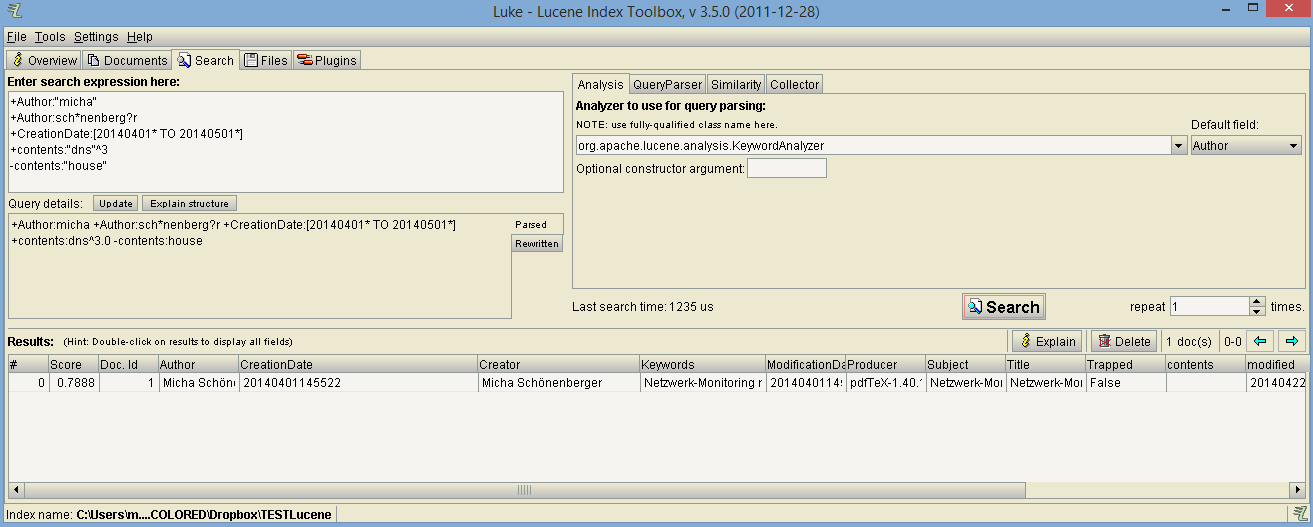
\includegraphics[width=1\textwidth]{Luke-Query.PNG} 
\caption[Such-Maske von Luke]{Such-Maske von Luke\\ Quelle: eigener Screenshot}
\label{fig:Luke-Query}
\end{figure}

\newpage
Anbei einige Beispiele, wie man den Syntax optimal einsetzen kann f�r sie Suche mit Luke/Lucene:
%==============  N E W  ==== S U B - S E C T I O N ==============%
\subsection{Felder}
\begin{tabular}[t]{|l|l|} \hline
contents:prtg & sucht das Wort \grqq prtg\grqq\ im Feld contents   \\ \cline{1-2}
Author:micha monitor & sucht das Wort \grqq micha\grqq\ im Feld Author, \\ 
 & das Wort \grqq netzwerk\grqq\ im default Feld \\ \cline{1-2}
contents:?mit prtg? & sucht die W�rter \grqq mit prtg\grqq\ als ganzes im Feld contents \\   \cline{1-2}
\end{tabular}
%==============  N E W  ==== S U B - S E C T I O N ==============%
\subsection{Wildcard Suche}
\begin{tabular}[t]{|l|l|} \hline
pr?g	& Das ? ersetzt einen einzelnen Charakter. So wird hier \\
 & z.B. nach ?prtg?, aber auch nach ?prag? gesucht \\ \cline{1-2}
bildschirm* & * steht f�r beliebig viele Zeichen (0 bis x) .\\
& Suche nach z.B. \grqq bildschirmeingabe\grqq\ oder \grqq bildschirme\grqq\\ \cline{1-2}
ver*en & * steht auch hier f�r beliebige Zeichen (0 bis x)\\
& Suche nach z.B. \grqq verwerfen\grqq\, \grqq verwalten\grqq\  oder \grqq veruntreuen\grqq \\ \cline{1-2}
\end{tabular}
 
Grunds�tzlich gilt: * und ? d�rfen nicht am Anfang der suche sein. (bei Luke gibt es eine Einstellung, mit der man * am Anfang erlauben kann)
%==============  N E W  ==== S U B - S E C T I O N ==============%
\subsection{Fuzzy Suche}
Die Fuzzy Suche basiert auf dem Levenshtein Distanz Algorithmus\footnote{siehe \url{http://www.levenshtein.de/}}, auf welchen hier nicht eingegangen wird.\\
Um eine Fuzzy Suche durchzuf�hren, wird mit der Tilde (~) gearbeitet.

\begin{tabular}[t]{|l|l|} \hline
roam~ & Sucht �hnliche W�rter zu roam \\ \cline{1-2}
roam~0.8 & Gibt die gesuchte �hnlichkeit an [0-1]. Je gr�sser die Zahl, desto �hnlicher. \\ \cline{1-2}
\end{tabular}



%==============  N E W  ==== S U B - S E C T I O N ==============%
\subsection{Proximity Suche (Nachbarschaftliche)}
Lucene erlaubt es, zwei W�rter in einer bestimmten Distanz zu suchen.

\begin{tabular}[t]{|l|l|} \hline
 \multirow{2}{3.5cm}{\grqq prtg monitor\grqq \textasciitilde10} &  Sucht die W�rter \grqq prtg\grqq \ und \grqq monitor\grqq  \\   
 & mit einem maximalen Abstand von 10 W�rtern\\ \cline{1-2}
\end{tabular}

%==============  N E W  ==== S U B - S E C T I O N ==============%
\subsection{Range Suche (Bereichssuche)}
Lucene erlaubt es, zum Beispiel Daten in einem bestimmten Bereich zu suchen.

\begin{tabular}[t]{|l|l|} \hline
 \multirow{2}{5.75cm}{modified:[20140501 TO 20140515]}&  Sucht eine Datei mit einem �nderungsdatum \\
 & zwischen dem 01.05.2014 und 15.05.2014\\ \cline{1-2}
 
  \multirow{2}{5.75cm}{Title:\{Anton TO Max\}}&  Sucht eine Datei mit dem Titel \\
 & zwischen Anton und Max (alphabetisch)\\ \cline{1-2}
 \end{tabular}

%==============  N E W  ==== S U B - S E C T I O N ==============%
\subsection{Boosting Suche (verst�rktes Suchen)}
Lucene erlaubt es, gewissen Suchbegriffen eine st�rkere Gewichtung zu verleihen. Durch diesen Boost wird das Ergebnis die Relevanz der gefundenen Dateien ver�ndert.

\begin{tabular}[t]{|l|l|} \hline
 \multirow{2}{5.75cm}{prtg\^\ 4 monitoring}&  Sucht eine Datei mit \flqq prtg\frqq \ und \flqq monitoring\frqq \\
 & wobei \flqq prtg\frqq \ 4-fach gewertet wird.\\ \cline{1-2}
  \end{tabular}


%==============  N E W  ==== S U B - S E C T I O N ==============%
\subsection{Boolsches Suchen}
Ganz wichtig beim Suchen sind die verschiedenen Verkn�pfungen der eingegebenen Suchbegriffe. Erlaubt sind AND, +, NOT, -

\begin{tabular}[t]{|l|l|} \hline

prtg OR monitor & Sucht entweder nach \flqq prtg\frqq \ oder nach \flqq monitor\frqq \\  \cline{1-2}
 \multirow{2}{4cm}{prtg AND monitor} & Sucht nach  \flqq prtg\frqq \ und nach \flqq monitor\frqq . Beide\\
 & W�rter m�ssen im selben Dokument enthalten sein.\\  \cline{1-2}
 
  \multirow{2}{4cm}{prtg NOT monitor} & Sucht ein Dokument, in welchem \flqq prtg\frqq \ vorkommt, \\
   & \flqq monitor\frqq \ aber nicht.\\ \cline{1-2}
  \multirow{2}{4cm}{NOT prtg} & NOT darf nicht mit nur einem Wort verwendet werden.\\
  & Das Resultat wird hier leer sein.\\ \cline{1-2}
  \end{tabular}
  
  
Anstelle von AND kann auch \&\& oder + verwendet werden.\\
Anstelle von NOT kann auch ! oder - verwendet werden.\\



Quelle: \cite{Luke_Query}


















